\documentclass[fontsize=12pt, paper=a4, headinclude, twoside=false, parskip=half+, pagesize=auto, numbers=noenddot, plainheadsepline, open=right, toc=listof, toc=bibliography]{scrreprt}
% PDF-Kompression
\pdfminorversion=5
\pdfobjcompresslevel=1

% Allgemeines
\usepackage[automark]{scrpage2} % Kopf- und Fußzeilen
\usepackage{amsmath,marvosym} % Mathesachen
\usepackage[T1]{fontenc} % Ligaturen, richtige Umlaute im PDF
\usepackage[utf8]{inputenc}% UTF8-Kodierung für Umlaute usw
\usepackage[verbose]{wrapfig}

% Schriften
\usepackage{mathpazo} % Palatino für Mathemodus
%\usepackage{mathpazo,tgpagella} % auch sehr schöne Schriften
\usepackage{setspace} % Zeilenabstand
\onehalfspacing % 1,5 Zeilen

% Schriften-Größen
\setkomafont{chapter}{\Huge\rmfamily} % Überschrift der Ebene
\setkomafont{section}{\Large\rmfamily}
\setkomafont{subsection}{\large\rmfamily}
\setkomafont{subsubsection}{\large\rmfamily}
\setkomafont{chapterentry}{\large\rmfamily} % Überschrift der Ebene in Inhaltsverzeichnis
\setkomafont{descriptionlabel}{\bfseries\rmfamily} % für description Umgebungen
\setkomafont{captionlabel}{\small\bfseries}
\setkomafont{caption}{\small}

% Sprache: Deutsch
\usepackage[german]{babel} % Silbentrennung

% PDF
\usepackage[english,pdfauthor={Adrian Kreskowski},  pdfauthor={Adrian Kreskowski}, pdftitle={Hardware-Assisted High-Quality Compression-Domain Rendering of Time-Varying Volumetric Data Sets}, breaklinks=true,baseurl={}]{hyperref}
\usepackage[final]{microtype} % mikrotypographische Optimierungen
\usepackage{url}
\usepackage{pdflscape} % einzelne Seiten drehen können

% Tabellen
\usepackage{multirow} % Tabellen-Zellen über mehrere Zeilen
\usepackage{multicol} % mehre Spalten auf eine Seite
\usepackage{tabularx} % Für Tabellen mit vorgegeben Größen
\usepackage{longtable} % Tabellen über mehrere Seiten
\usepackage{array}

%  Bibliographie
%\usepackage{bibgerm} % Umlaute in BibTeX

% Tabellen
\usepackage{multirow} % Tabellen-Zellen über mehrere Zeilen
\usepackage{multicol} % mehre Spalten auf eine Seite
\usepackage{tabularx} % Für Tabellen mit vorgegeben Größen
\usepackage{array}
\usepackage{float}

% Bilder
\usepackage{graphicx} % Bilder
\usepackage{color} % Farben
\usepackage{caption}
\usepackage{subcaption}
\graphicspath{{images/}}
\DeclareGraphicsExtensions{.pdf,.png,.jpg} % bevorzuge pdf-Dateien
%\usepackage{subfigure} % mehrere Abbildungen nebeneinander/übereinander
%\newcommand{\subfigureautorefname}{\figurename} % um \autoref auch für subfigures benutzen
\usepackage[all]{hypcap} % Beim Klicken auf Links zum Bild und nicht zu Caption gehen

% Bildunterschrift
\setcapindent{0em} % kein Einrücken der Caption von Figures und Tabellen
\setcapwidth{0.9\textwidth}
\setlength{\abovecaptionskip}{0.2cm} % Abstand der zwischen Bild- und Bildunterschrift

% Quellcode
\usepackage{listings} % für Formatierung in Quelltexten
\definecolor{grau}{gray}{0.25}
\lstset{
	extendedchars=true,
	basicstyle=\tiny\ttfamily,
	%basicstyle=\footnotesize\ttfamily,
	tabsize=2,
	keywordstyle=\textbf,
	commentstyle=\color{grau},
	stringstyle=\textit,
	numbers=left,
	numberstyle=\tiny,
	% für schönen Zeilenumbruch
	breakautoindent  = true,
	breakindent      = 2em,
	breaklines       = true,
	postbreak        = ,
	prebreak         = \raisebox{-.8ex}[0ex][0ex]{\Righttorque},
}

% linksbündige Fußboten
\deffootnote{1.5em}{1em}{\makebox[1.5em][l]{\thefootnotemark}}

\typearea{14} % typearea am Schluss berechnen lassen, damit die Einstellungen oben berücksichtigt werden
% für autoref von Gleichungen in itemize-Umgebungen
\makeatletter
\newcommand{\saved@equation}{}
\let\saved@equation\equation
\def\equation{\@hyper@itemfalse\saved@equation}
\makeatother 


% Eigene Befehle %%%%%%%%%%%%%%%%%%%%%%%%%%%%%%%%%%%%%%%%%%%%%%%%%
% Matrix
\newcommand{\mat}[1]{
      {\textbf{#1}}
}
\newcommand{\todo}[1]{
      {\colorbox{red}{ TODO: #1 }}
}
\newcommand{\todotext}[1]{
      {\color{red} TODO: #1} \normalfont
}
\newcommand{\info}[1]{
      {\colorbox{blue}{ (INFO: #1)}}
}
% Hinweis auf Programme in Datei
\newcommand{\datei}[1]{
      {\ttfamily{#1}}
}
\newcommand{\code}[1]{
      {\ttfamily{#1}}
}




% bild mit defnierter Breite einfügen
\newcommand{\bild}[4]{
  \begin{figure}[!hxbt]
    \centering
      \vspace{1ex}
      \includegraphics[width=#2]{images/#1}
      \caption[#4]{\label{img.#1} #3}
    \vspace{1ex}
  \end{figure}
}

% bild mit defnierter Breite einfügen
\newcommand{\bildlatexplaced}[4]{
  \begin{figure}
    \centering
      \vspace{1ex}
      \includegraphics[width=#2]{images/#1}
      \caption[#4]{\label{img.#1} #3}
    \vspace{1ex}
  \end{figure}
}
% bild mit eigener Breite
\newcommand{\bilda}[3]{
  \begin{figure}[!hbt]
    \centering
      \vspace{1ex}
      \includegraphics{images/#1}
      \caption[#3]{\label{img.#1} #2}
      \vspace{1ex}
  \end{figure}
}

% bild mit eigener Breite
\newcommand{\bildfloatright}[4]{
\begin{wrapfigure}{r}{width=#2}
  \begin{center}
    \includegraphics[width=1.0\textwidth]{images/#1}
  \end{center}
  \caption[#4]{\label{img.#1} #3}
\end{wrapfigure}
}

% Bild todo
\newcommand{\bildt}[2]{
  \begin{figure}[!hbt]
    \begin{center}
      \vspace{2ex}
	      
\includegraphics[width=6cm]{images/todobild}
      %\caption{\label{#1} \color{red}{ TODO: #2}}
      \caption{\label{#1} \todotext{#2}}
      %{\caption{\label{#1} {\todo{#2}}}}
      \vspace{2ex}
    \end{center}
  \end{figure}
}



 % Importiere die Einstellungen aus der Präambel
% !TEX root = ./main.tex
% hier beginnt der eigentliche Inhalt
\DeclareUnicodeCharacter{00A0}{ }

\DeclareCaptionLabelFormat{bold}{\textbf{(#2)}}
\captionsetup{subrefformat=bold}

\usepackage{appendix}
\usepackage[utf8]{inputenc}
\usepackage{ltablex}
%\usepackage[linesnumbered,ruled]{algorithm2e,algpseudocode}
\usepackage{algorithm2e,algpseudocode}

\usepackage[table]{xcolor}
\usepackage{pgfplots}
\pgfplotsset{width=10cm,compat=1.9}
\usepackage{amsmath}
\usepackage{pbox}

\hypersetup{hidelinks}


\begin{document}
\pagenumbering{Roman} % große Römische Seitennummerierung
\pagestyle{empty}

% Titelseite //////////////////////////////////////////
\clearscrheadings\clearscrplain

\begin{flushleft}
\begin{normalsize}
Bauhaus-Universität Weimar\\
Fakultät Medien \\
Studiengang Medieninformatik
\vspace{3mm}
\end{normalsize}
\end{flushleft}

\begin{center}
\vspace{20mm}
\begin{LARGE}
Visualization of Large Text Corpora 
%Temporal Interpolation and Spatio-Temporal Compression of Large Time-Varying Volume Data-Sets\\
\end{LARGE}
\vspace{20mm}
\begin{LARGE}
Bachelorarbeit
\end{LARGE}\\
\vspace{0.4cm}
\vspace{2 cm}

\vspace{1 cm}
\begin{flushleft}Giuliano Castiglia \hfill Matrikelnummer 110656\\
geb. am: 8. Oktober 1991 in Neapel
\end{flushleft} 

\vspace{0.5 cm}

\begin{flushleft}
1. Gutachter: Prof. Dr. Bernd Fröhlich\\
2. Gutachter: tba\\
\end{flushleft}

\vspace{1.5cm}
\begin{flushleft}
Datum der Abgabe: 4. September 2017
\end{flushleft}
\end{center}
\clearpage
\pagestyle{useheadings} % normale Kopf- und Fußzeilen für den Rest
\renewcommand*\contentsname{Table of Contents}

% ===============================================================

% % Eidesstattliche Erkl"arung 
% \addchap{Eidesstattliche Erklärung}

% Hiermit versichere ich, dass ich die Bachelorarbeit selbstständig verfasst und keine anderen als die angegebenen Quellen und Hilfsmittel benutzt habe, alle Ausführungen, die anderen Schriften wörtlich oder sinngemäß entnommen wurden, kenntlich gemacht sind und die Arbeit in gleicher oder ähnlicher Fassung noch nicht Bestandteil einer Studien- oder Prüfungsleistung war. 
 
% \vspace{3cm}
% Weimar, 10$^{\text{th}}$ February 2017

% \vspace{1cm}
% \noindent\rule{5cm}{0.4pt}\\
% GIULIANO CASTIGLIA

% \clearpage

% ===============================================================

% \addchap{Zusammenfassung}
% \todo{Write at last brief summarization of thesis}

% ===============================================================

\tableofcontents
%\listoffigures
%\listoftables


% ===============================================================

% richtiger Inhalt
\cleardoublepage
\pagenumbering{arabic} % ab jetzt die normale arabische Nummerierung


\chapter{Einleitung}
\label{chap:einleitung}
% !TEX root = ../main.tex
% Einleitung

Einleitung in InfoVis\\
Relevanz von Informationsvisualisierung\\
Bezug auf das vorangegangene Projekt Visual Text Analytics\\
Eine gebite ind er Einleitung:\\
einmal eine Abtrakte Motivation -> Darstellung Kategorienbaum + "Ahnlichkeiten

Motivation aus dem vorg"anger Projekt -> konkreter Bezug auf fehlende eigenschaften und Erkenntnisse
defacto die einzige Visualisierung f"ur den Kategoriebaum der Wikipedia


\section{Motivation}
\begin{itemize}
  \item Bedeutung des Wikipediadatensatzes
  \item Kritikpunkte im Projekt Visual Text Analytics
  \begin{itemize}
    \item statische Layout
    \item fehlende M"oglichkeit zur Exploration der Daten
    \item "Ubersicht der Visualisierung ist sehr undurchsichtig
    \item Schwierigkeiten beim nachvollziehen der Verbindungen der Artikel untereinander
    \item "Anderung des Schwellwertes f"ur "Ahnlichkeiten -> zu viele Kanten
    \item fehlende M"oglichkeit die Auswahl an Artikel einzuschr"anken
    \item Unterst"utzende Funktion zum Zusammenfassen von mehreren Artikel -> Kategorien, Cluster
    \item Artikelcluster mit viele "Ahnlichkeiten zueinander sind schwer zu lesen
    \item Kategorienbaum nur unzureichend als Unterzt"utzung neben den Artikeln
  \end{itemize}
\end{itemize}


\section{Ziel}
\begin{itemize}
    \item Verbesserung des Verst"andnisses des "Ahnlichkeitsma"ses
    \item Darstellung der Hierarchie von Kategorien
    \begin{itemize}
      \item Konstruktion eines Kategorienbaum mit der M"oglichkeit der Exploration
    \end{itemize}
    \item Interaktive Visualisierung
    \begin{itemize}
      \item "Anderung des Schwellwertes zur Laufzeit
    \end{itemize}
    \item Exploration der Daten
    \item Bezug zu anderen Datens"atzen: Authoren, Editierungen, etc.
\end{itemize}














% % ////////////////////////////////////
% \begin{figure}[H]
%     \centering
%     \begin{subfigure}[b]{0.96\textwidth}
%         \includegraphics[width=\textwidth]{images/01_introduction/motivation_temporal_superresolution_one.pdf}
%         \caption{3D video playback rate matching the low recording rate}
%         % \label{subfig:playback_rate_matching}
%     \end{subfigure}

% 	\vspace{1.0cm}

%     \begin{subfigure}[b]{0.96\textwidth}
%         \includegraphics[width=\textwidth]{images/01_introduction/motivation_temporal_superresolution_two.pdf}
%         \caption{3D video playback matching the video encoding standards to ensure persistence of fluid motion}
%         % \label{subfig:playback_rate_higher}
%     \end{subfigure}
%     \caption[Concept of Temporal Super Resolution in a 3D Video Player]{In this Figure, two different playback rates for a low frame rate recording of a 3D volume sequence is presented. The tick marks on the black arrows indicate the position of recorded frames. The blue arrows indicate the playback rate that matches the recording \subref{subfig:playback_rate_matching} and an increased playback rate \subref{subfig:playback_rate_higher} using temporal interpolation to provide the viewer with a impression of fluid motion. }
%     % \label{fig:temporal_superresolution}
% \end{figure}

%  \cite{VillanuevaEtAl:2016}

\chapter{Related Work}
\label{chap:related_work}
% !TEX root = ../main.tex

% Related Work
\section{Wikipedia Visualisierungen}
\section{Graphen und B"aume}
\section{Radiales Layout}










\chapter{Daten}
\label{chap:daten}
% !TEX root = ../main.tex
% Daten

\todo{Martin fragen nach Namen f"ur die "`Matrix"'}

Dieser Teil der Arbeit besch"aftigt sich mit der Struktur der genutzten Datens"atze.
Es wird erl"autert welche Schritte ben"otigt werden um die Datens"atze zu erstellen und nach welchen Regel sie formatiert sind.
Au"serdem wir beschrieben, welche Schritte n"otig sind um die n"otigen Informationen f"ur die Visualisierung zu extrahieren.
Bei den genutzte Datens"atzen handelt es sich um einen Wikipedidump im XML Format und um eine sp"arlich besetzte Adjazenzmatrix.
Beide Datens"atze sind sehr unterschiedlich in ihrer Struktur, als auch ihrem Inhalt und Umfang.
In den letzten beiden Teilen dieses Kapitels wird genauer auf den Aufbau der Datenbank eingegangen und wie die Daten w"ahren der Laufzeit des Programms bearbeitet werden.

%NOTE: vllt groesse martin erste simMatrix
\begin{table}
\centering
% \begin{center}
\begin{tabular}{l r}
  \hline
  Datensatz & Gr"o"se \\
  \hline
  Wikipediadump & 54 GB \\
  "Ahnlichkeitsmatrix & 642 GB \\
  \hline
\end{tabular}
% \end{center}
\caption{Gr"o"se der Datens"atze in GB}
\label{dataset-size}
\end{table}


\section{"Ahnlichkeitsmatrix}
Der Gr"o"sere von beiden Datens"atzen ist die d"unn besetzte Matrix.
In der Matrix werden die berechneten "Ahnlichkeitswerte zwischen zwei Artikeln gespeichert.

In der "Ahnlichkeitsmatrix nach \cite{riehmann2016visualizing} werden alle Artikel der Wikipedia mit 
In zwei vorangegangen Projekten wurde



\begin{itemize}
    \item Bezugname Arbeit von Potthast
    \item Bezugnahme zur Thesis von Tristan Licht
    \item Vergleich der zwei Datens"atze

    \begin{itemize}
      \item Verwendetes "Ahnlichkeitesma"s
      \item "Ahnlichkeit von Paragraphen
      \item Daten "uber die "Ahnlichkeiten (Anzahl)
    \end{itemize}
    \item Inhalt der Matrix
    \begin{itemize}
      \item
    \end{itemize}
\end{itemize}
 % =================================================



\section{Wikipedia XML Dump}
\begin{itemize}
    \item Datenstruktur des Wikipediakorpus
    \item Notwendige Metainformationen aus dem Korpus
    \item Struktur Kategoriebaum
\end{itemize}
 % =================================================



\section{Datenbankentwurf}
\begin{itemize}
    \item Erl"auterung der Datenbankstruktur
\end{itemize}
 % =================================================


\section{Ablauf der Datenverabeitung}
\begin{itemize}
    \item Aufbereitung der Rohdaten: S"auberung, Formatierung
    \item Erstellung der Datenbank
\end{itemize}
 % =================================================


\chapter{Visualisierung}
\label{chap:visualization}
% !TEX root = ../main.tex
% Visualisierung

% Kapitel \ref{chap:daten} gibt einen "Uberblick "uber gr"o"se und Struktur der genutzten Datens"atze um nachvollziehen zu k"onnen welche Daten visualisiert werden.
In diesem Kapitel wird auf die gewählte Darstellung von Kategorien eingegangen und welche Interaktionsmöglichkeiten die Visualisierung bietet.
Darüber hinaus wird verdeutlicht, welche nicht sichtbaren Veränderungen während der Laufzeit des Programms an den Daten vorgenommen werden.
In diesem Kapitel werden die beschriebenen Datensätze aus Kapitel \ref{chap:daten} weiter dargelegt und mit ihrer visuellen Repräsentation verknüpft.

Im Gegensatz zur Visualisierung aus dem Projekt \emph{Visual Text Analytics} stehen die Verbindungen zwischen den Kategorien im Mittelpunkt der angestrebten Darstellung.
Der Ansatz aus dem vorangegangenen Projekt, möglichst viele Artikel und ihre Ähnlichkeiten abzubilden, führt zu einer unüberschaubaren Menge an Vergleichen, die wiederum in einer Undurchsichtigkeit der dargestellten Elemente resultiert (\emph{visual clutter}).
In dieser Arbeit wird ein neuer Ansatz verfolgt, welcher sich auf Kategorien fokussiert.
Die Kategorien sollen einen abstrakteren Zugang zu den Artikeln schaffen, die Übersichtlichkeit stärken und die Auswahl an Artikeln auf ein Themengebiet beschränken.

%  Vorhaben, eine geeignete Darstellungsform der Kategorienstruktur zu finden, folgend wird diese Struktur analysiert.
% % Die Voraussetzung dafür ist die Analyse der Kategorienstruktur der Wikipedia 
Der Grundgedanke der Arbeit liegt in der Annahme, die Kategorienstruktur als Hierarchie von Abstraktionsebenen zu interpretieren.
Diese Annahme soll durch eine Analyse der Kategorienstruktur überprüft werden.
Auf der Wikipedia-Seite \emph{Main Topic Classifications} \footnote{\url{https://en.wikipedia.org/wiki/Category:Main_topic_classifications}} wird darauf hingewiesen, dass die Kategorienstruktur nicht als strikt hierarchisch verstanden werden soll.
Daraus lässt sich schließen, dass Kategorien in einem Graph miteinander verbunden sind.
Die genauere Betrachtung der Beziehungen zwischen den Kategorien verdeutlicht ihre Eigenschaft.
Besteht eine Verbindung zwischen zwei Kategorien, werden diese jeweils in der anderen Kategorie als Unterkategorie oder als Oberkategorie eingetragen. 
Daraus lässt sich folgern, dass der Graph, bestehend aus Verbindungen zwischen Kategorien, ein gerichteter Graph ist und so einer gewissen Ordnung folgt.

Nun soll, ausgehend von einem bestimmten Stammverzeichnis, ein Pfad von Unterkategorien beispielhaft erkundet werden.
Dies soll die verschiedenen Stufen der Abstraktion eines Themengebiets anhand von Unterkategorien verdeutlichen.
Die Analyse der Wikipedia-Seite der Kategorie \emph{Main topic classifications} und deren Unterkategorien zeigt, dass die Kategorien, die näher zum gewählten Stammverzeichnis liegen, Themengebiete eher umfassend beschreiben.
Die Kategorien, die weiter vom Stammverzeichnis entfernt sind, umschreiben hingegen einen Gegenstand ausführlicher.
Auf Grund dieser Beobachtung wird davon ausgegangen, dass die Kategorienstruktur einer thematischen Ordnung bzw. einer thematischen Hierarchie folgt. 
Diese Ordnung der Kategorien wird noch einmal in Abbildung \ref{fig:main-topic-tree} verdeutlicht.

\begin{figure}
    \centering
    \begin{tikzpicture}
    \end{tikzpicture}
    \caption{Ausschnitt der Kategorienstruktur ausgehend von der Kategorienseite \emph{Main topic classifications}}
    \label{fig:main-topic-tree}
\end{figure}

Die Konstruktion eines Baumes, der die Hierarchie abbilden soll, ist kein triviales Problem, folgend werden zwei unterschiedliche Ansätze erklärt dieses Problem zu lösen.
Die Ansätze unterscheiden sich dabei nicht wesentlich von einander.
Aus den vorangegangenen Beobachtungen lässt sich folgendes schließen:\\
Die Kategorien untereinander folgen einer Ordnung, diese wird durch die gerichteten Verbindungen zwischen Kategorien abgebildet.
Diese Feststellung bildet die Basis um aus dem gerichteten Graphen einen Baum zu konstruieren, der die Hierarchie der Kategorien abbildet.\\
Weiterhin besteht die Schwierigkeit, die Konstruktion von Schleifen für einen Kategorienbaum aus dem Kategoriengraph heraus zu verhindern und somit zu entscheiden welche Kanten aus dem gerichteten Graphen im Baum bestehen bleiben.
Als Ansatz soll ausgehend von eine gewählten Startkategorie der gerichtete Graph mit einer Breitensuche traversiert werden.
Dabei werden nur Knoten aus dem Graphen dem Baum hinzugefügt, die nicht bereit im Baum abgebildet sind.
Die Knoten einer Ebene werden nur mit dem Knoten verbunden, von dem eine gerichtete Kante aus sie ausgeht.
Auf diese Art soll gewährleistet werden das keine Schleifen während der Konstruktion des Baumes entstehen.
In Kapitel \nameref{chap:Implementierung} wird der verwendete Algorithmus, welcher aus dem gerichteten Graphen ein Baumdiagramm konstruiert, weiter geschildert.\\

% schleife erklären
% Baumkonstruktion schleifen Problem, keine Feste Hierarchie
% Aus diesem Grund wird beispielhaft versucht, eine  Kategorienhierarchie zu konstruieren.
% In einem weiteren Schritt wird der gerichtete Graph traversiert und die Kategorien werden in Form eines Baums konstruiert. Dabei sollen die Kanten verworfen werden, welche die Kategorien einer Ebene mit einer höheren Ebene verbinden. 

Der erste Ansatz versucht einen Kategorienbaum für \emph{alle} Wikipedia-Kategorien zu erstellen.
Für einen vollständigen Kategorienbaum wird ein Stammverzeichnis gesucht, das zwei Eigenschaften erfüllt:\\
Ein globales Stammverzeichnis sollte in den von ihr ausgehenden Unterkategorien ausschließlich Kategorienseiten oder Artikelseiten eingetragen haben.
Zusätzlich sollte ein Stammverzeichnis so gewählt werden, dass möglichst viele Themengebiete direkt oder in Unterkategorien enthalten sind.
Die Wikipedia markiert die Kategorie \emph{Contents} \footnote{\url{https://en.wikipedia.org/wiki/Category:Contents}} als Stammverzeichnis aller Kategorienseiten.
Diese Seite ist gleichwohl ungeeignet für die Nutzung als Stammverzeichnis, da in ihr auch Kategorien aus Namensräumen außerhalb der Artikelseiten eingetragen sind.
Ausgehend von der Stammkategorie \emph{Contents} über die Unterkategorie \emph{Articles}  gelangt man zur Unterkategorie \emph{Main topic classifications}.
In ihren Unterkategorien sind hauptsächlich Artikelseiten eingetragen. 
Die direkten Unterkategorien enthalten 22 unterschiedliche Themengebiete die den Inhalt der Wikipedia abbilden.
In dieser Arbeit wird die Kategorie \emph{Main Topic Classifications} \footnote{\url{https://en.wikipedia.org/wiki/Category:Main_topic_classifications}} als globales Stammverzeichnis für alle Kategorien gewählt.\\

Sucht ein Nutzer nach einer Kategorie, ist es nun möglich ihm einen Ausschnitt der vollständigen Hierarchie, von der gesuchten Kategorie aus beginnend, darzustellen.
Das Problem der dargestellten Hierarchie ist, dass es bestimmte Verbindungen mit der gesuchten Kategorie oder ihren Unterkategorie nicht dargestellt werden, weil sie in einem anderen Pfad der vollständigen Hierarchie abgebildet sind.
In Abbildung \ref{fig:two-trees} wird diese noch einmal verdeutlicht.

\begin{figure}
    \centering
    
\includegraphics{images/todobild.pdf}
    \caption{Es werden zwei Kategorienbaum für die Wurzelkategorie \emph{History angezeigt}, konstruiert mit den unterschiedlichen Anstäzen aus der \ref{chap:visualization}}
    \label{fig:two-trees}
\end{figure}

Der zweite Ansatz versucht diesen Fehler in der Darstellung einer Hierarchie aus dem gerichteten Graphen, zu mindern.
Sucht der Nutzer nach einer Kategorie wird, wie bereits am Anfang des Kapitels beschrieben mit der Breitensuche und festgelegten Bedingungen ein neuer Kategorienbaum konstruiert.
Diese unterscheidet sich vom Ausschnitt des Kategorienbaums der vollständigen Hierarchie aus dem ersten Ansatz, diese soll mit der Abbildung \ref{fig:two-trees} veranschaulicht werden.
Dabei ist die Anzahl an Verbindungen die im zweiten Kategorienbaum abgebildet werden an den tatsächlichen Verbindugnen des gerichteten Graphen für die Wurzelkategorie, als in dem Ansatz mit der vollständigen Hierarchie.
Dieser Kategorienbaum bildet eine genaueres Abbild der Hierarchie für die gewählte Wurzelkategorie ab.
Dabei sollte beachtet werden, dass die dargestellte Hierarchie immer nur eine Interpretation des gerichteten Graphen ist.

In beiden fällen wird jedoch mit der Hierarchie der Kategorien ein \emph{Top-Down}-Struktur \emph{\url{https://de.wikipedia.org/wiki/Top-down_und_Bottom-up}} modelliert, welche genutzt werden soll um Themengebiete zu erkunden.
In dem Abschnitt \ref{subchap: filter-vis} wird erklärt wie die \emph{Top-Down}-Exploration genutzt wird um auf Artikel zuzugreifen, dieser Ansatz spielt dabei die Grundlegende Rolle in der Selektion der Artikel.
In den folgenden Abschnitten wird auf die visuelle Umsetzung und Interkation der Arbeit eingegangen.

\begin{figure}
    \centering
    \begin{tikzpicture}
    \node[draw=red, very thick] (fig) at (3,3) {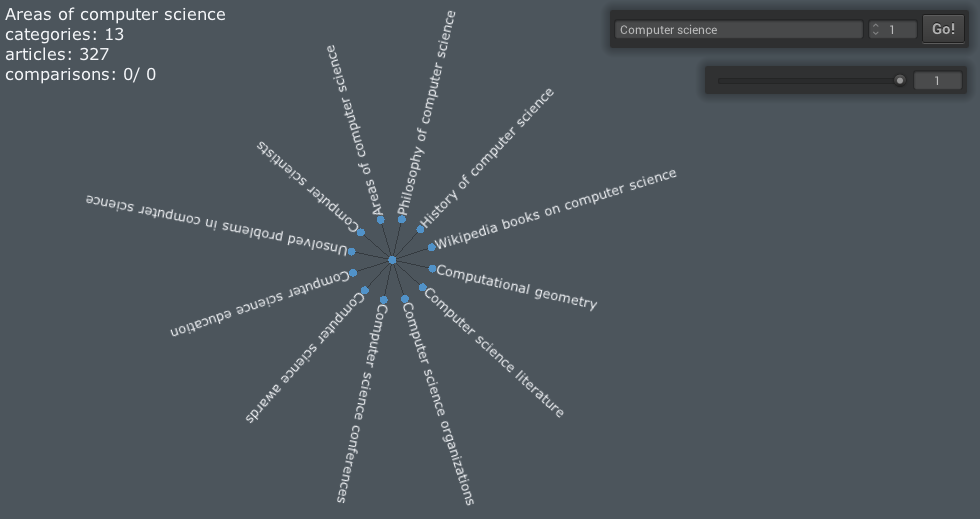
\includegraphics[width=\textwidth]{images/small-start-cs-lvl1.png}};
    \node[red, below] at (fig.south) {(a)};
    
    \node (one) at(-3.3,6.6) [rectangle, draw=red, very thick, inner sep=0pt, minimum width=3.9cm, minimum height=1.5cm]{};
    \node[red, below] at (one.south) {(b)};
    
    \node (two) at(8,6.9) [rectangle, draw=red, very thick, inner sep=0pt, minimum width=6.2cm, minimum height=.75cm]{};
    \node[red, above] at (4.5, 6.6){(c)};
    \node (three) at(8.8,6) [rectangle, draw=red, very thick, inner sep=0pt, minimum width=4.6cm, minimum height=.6cm]{};
    \node[red, below] at (three.south) {(d)};
    \end{tikzpicture}
    \caption{Darstellung der Kategorie \emph{Computer science} im Zentrum des radialen Graphen.
    Es sind die Unterkategorien mit einer Tiefe von eins mit der Stammkategorie verbunden und sichtbar.\\ (a) Hauptfenster, (b) zusammenfassende Statistik über vorhandene Daten, (c) Suchleiste, (d) Regler zur Änderung des Schwellwerts}
    \label{fig:small-start}
\end{figure}


\section{Layout} \label{subchap:layout}

In dieser Arbeit werden Ausschnitte der Kategorienstruktur der Wikipedia, welche sich insgesamt auf etwa $1.4$ Millionen Seiten beläuft, siehe Tabelle \ref{tab:xml-overview}, dargestellt.
Wie einleitend in diesem Kapitel beschrieben, werden die Kategorien der Wikipedia als hierarchischer Baum modelliert.
Die Veränderung der Baumdarstellung durch Hinzufügen von Knoten wird möglich gemacht. 
Es gibt verschiedene Möglichkeiten, Bäume anzuordnen. 
Bekannte Methoden sind die horizontale oder vertikale Ausrichtung von Baumdarstellungen.
Die enorme Menge an möglichen Kategorien, die dargestellt werden können, erfordert eine Methode, welche den vorhandenen Platz des Bildschirms voll ausschöpft und dabei die Anordnung von Knoten in einer vertretbaren Zeit berechnet.
Dabei wird die hierarchische Struktur eines Baumes abgebildet und die Veränderung der Darstellung durch Hinzufügen von weiteren Knoten ermöglicht.
Hierfür werden zwei Ansätze ausprobiert, welche nachfolgend erläutert werden.\\
Der erste Versuch wurde mit dem Algorithmus nach Fruchtermann et al. \cite{fruchterman1991graph} implementiert.
In dieser Arbeit wird eine Implementierung des Algorithmus' aus der Bibliothek der \emph{Boost Graph Library} \footnote{\url{http://www.boost.org/doc/libs/1_65_1/libs/graph/doc/index.html}} verwendet. Die Standardeinstellungen der Parameter des Algorithmus wurden beibehalten.
In diesem Versuch stellt sich heraus, dass die Berechnung der Knoten anhand eines physikalischen Modells ab einer gewissen Größe zu rechen- und zeitintensiv wird, sodass keine Interaktion mit der Darstellung möglich ist.
Ein weiteres Problem dieses Ansatzes ist die Positionierung der Knoten selbst.
Aus der Anordnung der Knoten nach dem Algorithmus von Fruchtermann et al. lässt sich schwer die hierarchische Struktur der Kategorien erkennen. 
Folglich ist der Algorithmus in dieser Form nicht optimal für die Darstellung des Kategorienbaums.
Auf Grund dieser Defizite wurde der Ansatz nicht weiter verfolgt.


Der zweite Ansatz versucht die Anordnung der Knoten des Kategorienbaums mit dem Algorithmus nach Eades \cite{eades1991drawing} zu realisieren.
Die Positionierung der Knoten erfolgt in einem polaren Koordinatensystem, dabei stellt die Wurzelkategorie den Ursprung dieses Systems dar.
Die Distanz und der Winkel zum Ursprung geben die Position eines Knotens an.
Der Algorithmus ermöglicht, dass jegliche Knoten einer Baumdatenstruktur als Wurzel für die Darstellung gewählt werden können. Anhand des ausgesuchten Knotens werden alle anderen Knoten in konzentrischen Ringen um den Wurzelknoten angeordnet.
Die Größe eines Sektors innerhalb des polaren Koordinatensystems, welche für einen Teilbaum belegt wird, ist davon abhängig, wie viele Knoten sich in dem Teilbaum befinden.
Ausschlaggebend für die Größe des Sektors ist dabei die Anzahl an Blattknoten des jeweiligen Teilbaums, siehe dazu Eades \cite[S.~15]{eades1991drawing}.
Der Algorithmus garantiert, dass die Anordnung des Baumes "planar" ist, also keine Überlappungen entstehen. \cite[S.~16]{eades1991drawing}.
Der Algorithmus erfüllt dabei die oben beschriebenen Voraussetzungen zur Darstellung des Kategorienbaumes.

% In dieser Arbeit wurde sich dazu entschlossen den Baum radial anzuordnen, da auf diese Weise gewährleistet wird, das der verfügbare Platz optimal genutzt wird. \footnote{\cite[Kapitel 5, p.~123]{lima2014book}}
% Die radiale Anordnung von Knoten und Kanten eines Baumes wird durch den Algorithmus nach Eades \cite{eades1991drawing} realisiert.
% Der Algorithmus muss dabei bestimmte Kriterien erfüllen, wie eine minimale Überlappung an Knoten und Kanten um eine Überhäufung wie im Vorgänger Porjekt zu vermeiden.
% Des Weiteren sollte der Algorithmus, 

Im Folgendem werden die Merkmale für Kreisdarstellungen aus der Taxonomie von Kreisen nach \cite[p.~57]{lima2017circle} genutzt, um den dargestellten Baum zu erläutern.\\
Wikipedia-Kategorien werden als Knoten in Form von blau gefärbten Kreisen dargestellt.
Verbindungen zwischen Wikipedia-Kategorien werden als Kanten in Form einer weißen Linie zwischen zwei Knoten dargestellt.
Nachfolgend wird der Begriff der Kategorie stellvertretend für die visuelle Form eines Knotens genutzt.
Die im Zentrum des Baumes liegende Kategorie repräsentiert die Stammkategorie und wird auch Wurzel genannt.
Alle dargestellten Knoten sind durch Kanten mit ihr verbunden.\\
Kategorien, die keine Unterkategorien besitzen, werden Blattkategorien genannt.
Die Distanz zwischen zwei Kategorien wird durch die Anzahl an Kanten festgelegt, die auf dem kürzesten Pfad zwischen den beiden Kategorien liegen.
Die Distanz einer Kategorie zur Wurzelkategorie wird auch als Tiefe bezeichnet.
Die Unterkategorien der Wurzelkategorie werden auf konzentrischen Ringen um die Wurzelkategorie angeordnet, welche auch als Kategorienebene bezeichnet wird.
Alle Unterkategorien einer Kategorienebene besitzen die gleiche Distanz zur Wurzelkategorie.
Die Anzahl an konzentrischen Ringen wird durch die tiefste dargestellte Kategorie bestimmt.
In Abbildung \ref{fig:small-start} wird die Visualisierung des Kategorienbaums mit einer Tiefe von eins dargestellt.

Die Größe einer Kategorie wird an der Anzahl an direkten Artikeln, die in der Kategorie eingetragen sind, gemessen.
Die Anzahl an Artikeln kann direkt auf die Größe des Knotens der Kategorie übertragen werden, wie in Abbildung \ref{fig:cat-size-direct} dargestellt.
Jedoch ist dies nicht wünschenswert, da so ein Teil der Elemente des Kategorienbaums überzeichnet wird.
Es muss eine Darstellungsform gefunden werden, bei der die Größe der Knoten einen festgelegten Wert nicht überschreitet. 
In Abbildung \ref{fig:cat-size-fixed} wird dies dargestellt.
Der Unterschied in der Größe der Knoten soll dem Nutzer eine weitere grundlegende Information über die Kategorien liefern: die Anzahl an Artikeln.
Dabei ist in Abbildung \ref{fig:cat-size-fixed} zu erkennen, dass es irritierend sein kann, dass nicht die Wurzelkategorie den größten Knoten darstellt.
Dies liegt daran, dass die Anzahl der Artikel nicht für die Unterkategorien einer Kategorie aufsummiert wird, da zuvor festgelegt wurde nur die direkten Artikel, welche in einer Kategorie eingetragen sind, zu zählen.

\begin{figure}
    \centering
    
\includegraphics{images/todobild.pdf}
    \caption{Die Anzahl der Artikel einer Kategorie wird direkt auf die Größe des Knotens der Kategorie übertragen}
    \label{fig:cat-size-direct}
\end{figure}

\begin{figure}
    \centering
    
\includegraphics{images/todobild.pdf}
    \caption{Durch eine festgelegte Funktion wird die Anzahl der Artikel einer Kategorie auf einen Wert abgebildet, welcher den Durchmesser des Knotens darstellt}
    \label{fig:cat-size-fixed}
\end{figure}

Die Beschriftung von Knoten ist notwendig, um die Knoten als Kategorien sichtbar zu machen und auch ohne Interaktion von Seiten des Nutzers bereits Informationen über den Kategorienbaum zu liefern.
Die Beschriftung erfolgt dabei für alle Blattkategorien der Darstellung und erlaubt eine Untersuchung der benachbarten Kategorien.
Für den Fall, dass eine bestimmte Kategorie von Interesse ist und sie expandiert wird, werden ihre Unterkategorien beschriftet.
In Abschnitt \ref{subchap:interaktion} wird die Interaktion durch eine Expansion weiter im Detail beschrieben.\\
Die Anordnung der Titel einer Kategorie erfolgt gleich dem Winkel des Knotens der Kategorie.
Durch diese Anordnung sind Knoten mit einem Winkel über 90 \textdegree und unter 270 \textdegree nur schwer leserlich oder gar kopfüber angeordnet.
Abschnitt \ref{subchap:interaktion} beschreibt eine Methode, die Lesbarkeit der Titel zu erleichtern.
% Die Wurzelkategorie im Zentrum des Kategorienbaums stellt dabei die gesuchte Kategorie 
% Lima beschreibt zwölf wesentliche Merkmale von Kreisen, dabei gehen wir nur auf Merkmale ein, die eine zentrale Rolle in der Visualisierung einnehmen.


\begin{figure}
    \centering
    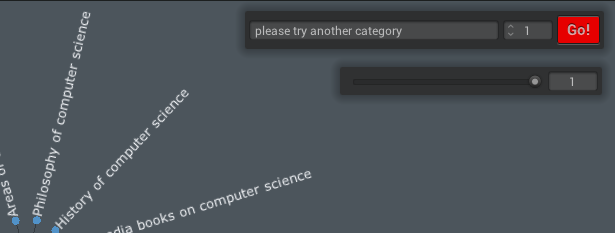
\includegraphics[scale=.5]{images/small-start-wrong-cat-1.png}
    \caption{Ein Nutzer hat bereits nach einer Kategorie gesucht, welche nicht in der Datenbank gefunden wurde. Der Nutzer wird durch die grafische Benutzeroberfläche aufgefordert, die Suche zu wiederholen.}
    \label{fig:wrong-cat}
\end{figure}

\section{Interaktion} \label{subchap:interaktion}
Die Interaktionen mit der Visualisierung lassen sich in zwei Gruppen einteilen. Ein Nutzer kann entweder mit der grafischen Benutzeroberfläche interagieren, wie in Abbildung \ref{fig:small-start} mit (b), (c) und (d) markiert, oder direkt mit den Inhalten im Hauptfenster, wie in der Abbildung mit (a) gekennzeichnet.
Nachfolgend werden die Möglichkeiten der Interaktion erläutert.

\paragraph{Grafische Benutzeroberfläche}
Element (b) aus Abbildung \ref{fig:small-start} ist ein passives Interaktionselement, da es Informationen nur anzeigt und nicht direkt durch den Nutzer verändert werden kann.
Das Element besteht aus vier Zeilen, welche Informationen über den aktuellen Kategorienbaum innerhalb des Hauptfensters (a) zur Verfügung stellen.
In der ersten Zeile wird der Titel der letzten Kategorie angezeigt, über die ein Nutzer den Mauszeiger platziert hat.
Hierdurch wird die Option geschaffen, Titel unbeschrifteter Kategorien zu erfahren.
Die zweite und dritte Zeile zeigen die aktuelle Anzahl der Kategorien und Artikel des Kategorienbaums an.
Es werden hierbei alle Artikel gezählt, welche direkt in Kategorienseiten eingetragen sind. Artikel, die mehrfach in unterschiedlichen Kategorien vorkommen, werden nur einmal berücksichtigt.
Die letzte Zeile des Elements (b) beschreibt die Anzahl an Artikelpaaren, die über dem festgelegten Schwellwert aus Element (d) liegen.
Die erste Zahl stellt dabei die Anzahl an Artikelpaaren dar, von denen beide Artikel einer Kategorie angehören, die auch im dargestellten Kategorienbaum zu finden ist.
Die zweite Zahl hingegen beschreibt die Artikelpaare, in denen nur einer der beiden Artikel in einer Kategorie des Kategorienbaums dargestellt wird.
Diese zwei Varianten von Artikelpaaren werden im Rahmen dieser Arbeit \emph{lokale} bzw. \emph{globale} Vergleiche von Artikeln genannt.
Auf dieses Konzept wird in Abschnitt \ref{subchap: filter-vis} weiter eingegangen.

Das Element (c) aus der Abbildung \ref{fig:small-start} ist Teil der grafischen Benutzeroberfläche und stellt eine Suchleiste für alle Kategorien der Wikipedia dar.
Die Suchleiste ist dabei aus drei Elementen aufgebaut, wie in Abbildung \ref{fig:wrong-cat} dargestellt.: dem Suchformular (1), dem Eingabefeld für die Tiefe (2) und einer Schaltfläche (3).\\
In der Suchleiste kann der Name einer möglichen Kategorie als Suchbegriff eingegeben werden.
Betätigt ein Nutzer nach der Eingabe einer gesuchten Kategorie die Schaltfläche "`Go!"', wird eine Suchanfrage mit dem eingegebenem Begriff an die Datenbank weitergeleitet.
Existiert keine Kategorie mit dem eingegebenen Begriff, wird die Schaltfläche "'Go!"` rot gefärbt und der Nutzer aufgefordert, eine andere Kategorie einzugeben, siehe Abbildung \ref{fig:wrong-cat}.
Existiert die Kategorie allerdings in der Datenbank, wird ein Kategorienbaum nach den festgelegten Parametern gezeichnet.
Der im Eingabefeld eingetragene Tiefen-Wert legt dabei die Anzahl der Ebenen fest.
Die gesuchte Kategorie wird zum Zentrum der Darstellung.
Das Feld für die Tiefe des Kategorienbaums kann durch Eingabe des Nutzers verändert werden.
Die Eingabe einer Zahl wird durch die Tastatur oder über die Pfeile im Eingabefeld ermöglicht.
Mit dem Tiefen-Wert wird die maximale Tiefe des Kategorienbaums, bis zu welcher die Blattkategorien mit einem niedrigerem Tiefenwert expandiert werden sollen, festgelegt.
Sollten Unterkategorien mit einem höheren Tiefenwert in der Darstellung angezeigt werden, betrifft sie diese Interaktion nicht.
Demzufolge ist die Distanz zwischen Blattkategorien und der Wurzelkategorie mindestens so groß wie die eingegebene Tiefe.
Die Expansion der Blattkategorien wird durch Betätigung der Schaltfläche "`Go!"' ausgeführt.
Dabei bleiben bereits gezeichnete Kategorien der Visualisierung unverändert, sofern sie tiefer als die Eingabetiefe sind.

Das andere Element der grafischen Benutzeroberfläche ist der Regler, mit dem ein Schwellwert für Ähnlichkeiten festgelegt wird.
Dieser wird in Abbildung \ref{fig:small-start} mit (d) gekennzeichnet.
Das Element besteht dabei aus zwei Feldern, einem Schieberegler und einem Zahlenfeld, an dem der eingestellte Wert abgelesen werden kann.
Der Schieberegler stellt dabei die Mindestgröße ein, die der Ähnlichkeitswert zwischen zwei Artikeln überschreiten muss um dargestellt zu werden.
Artikelpaare mit einem Ähnlichkeitswert, der niedriger ist als der Schwellwert, werden nicht in Betracht gezogen.
% Die Veränderung des Schiebereglers ändert neben dem Schwellwert auch die Farbe der Knoten von blau nach gelb.
Der Schieberegler beeinflusst aber nicht nur die Selektion der Daten aus der Ähnlichkeitsmatrix, sondern auch das Erscheinungsbild der Visualisierung.
Kategorien werden gelb gefärbt, wenn die darin eingetragenen Artikel eine Ähnlichkeit zu einem Artikel aus einer bereits dargestellten Kategorie aufweisen, die höher oder gleich dem Schwellwert ist.
Der Schieberegler zeigt folglich die Kategorien an, unter denen Artikelpaare mit einer Ähnlichkeit über oder gleich dem Schwellwert eingetragen sind.
Diese Form der Selektion der dünn besetzten Ähnlichkeitsmatrix, nennen wir horizontale Filterung.
Abbildung \ref{fig:simM-threshold-cat} soll dies verdeutlichen.
\begin{figure}
    \centering
    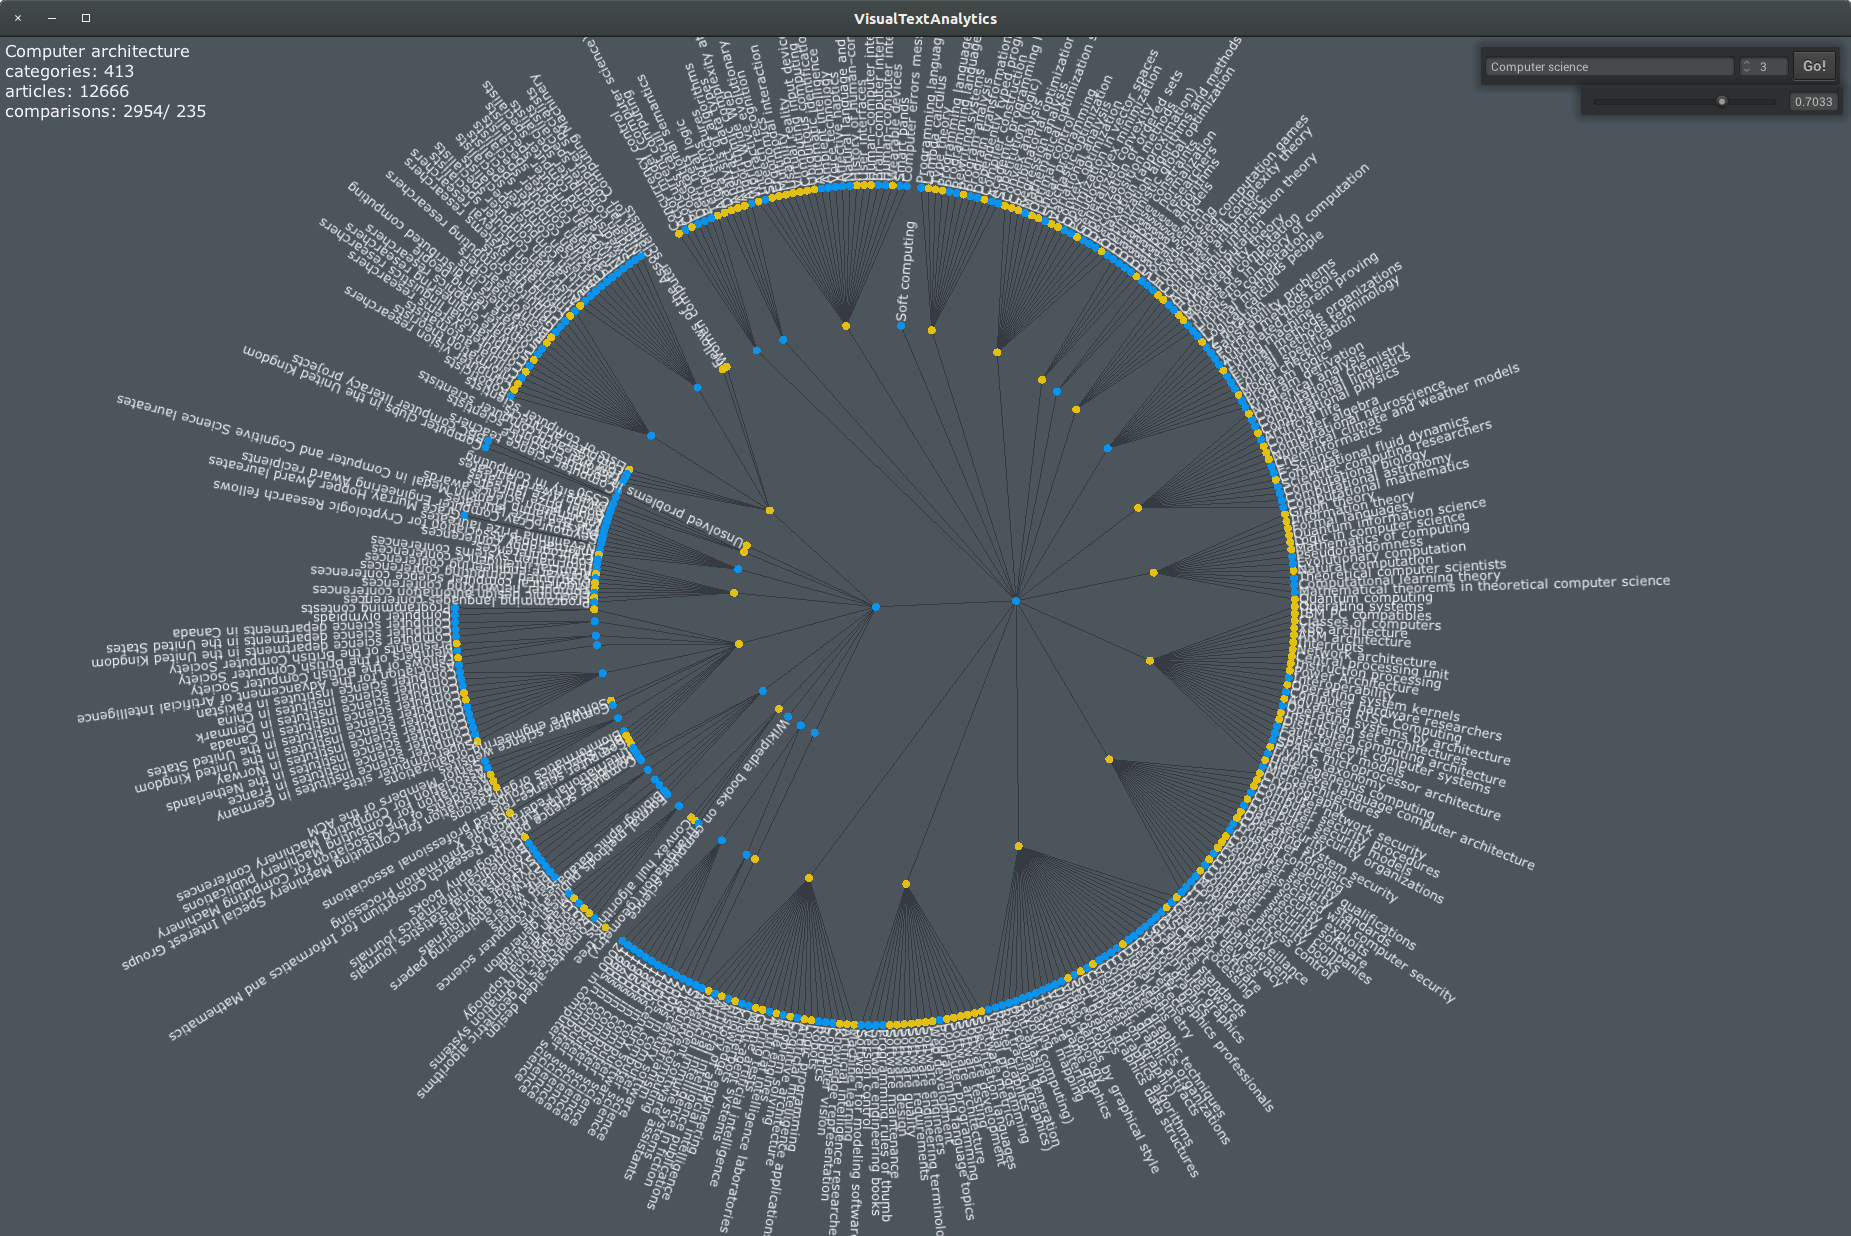
\includegraphics[width=\textwidth]{images/threshold-7033-lvl3}
    \caption{Färbung von Kategorien über dem Schwellwert, Eingabe des Schwellwerts}
    \label{fig:threshold-cat}
\end{figure}


\paragraph{Hauptfenster}
Als Hauptfenster wird der Bereich bezeichnet, der in Abbildung \ref{fig:small-start} mit (a) markiert ist.
Davon ausgenommen sind die Elemente der grafischen Benutzeroberfläche.
Im Hauptfenster wird der Kategorienbaum als Knoten- und Kantendiagramm dargestellt
Der Kategorienbaum steht im Mittelpunkt der Visualisierung.
Es bestehen verschiedene Möglichkeiten, mit dem Kategorienbaum zu interagieren:\\ 1. die Verschiebung und das Vergrößern, 2. die Rotation und 3. die Erweiterung des Kategorienbaums.\\
Durch die Verschiebung und die Vergrößerung der Darstellung des Kategorienbaums wird dem Nutzer die Möglichkeit geschaffen den Kategorienbaum frei zu platzieren und ausgewählte Knoten zu fokussieren.
Durch die radiale Anordnung der Kategorien und ihre Beschriftung in radialer Ordnung ist es möglich, den Kategorienbaum um die Wurzelkategorie zu drehen.
Bei gedrückt gehaltener "`Strg"'-Taste und gleichzeitiger Drehung am Mausrad, dreht auch sich der Kategorienbaum.
Diese Interaktion soll dem Nutzer ermöglichen, den Kategorienbaum so ausrichten zu können, dass er im Stande ist, die Beschriftung einer bestimmten Kategorie zu lesen.
\begin{figure}
    \centering
    \begin{tikzpicture}
    \matrix (m) [matrix of nodes, nodes in empty cells]
    {
        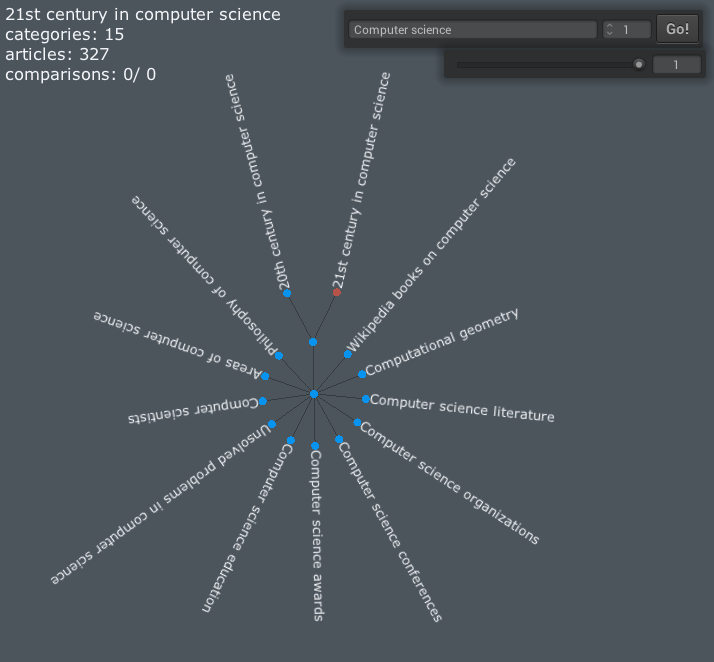
\includegraphics[scale=.21]{images/rotation-hist-1}&[3mm]&
        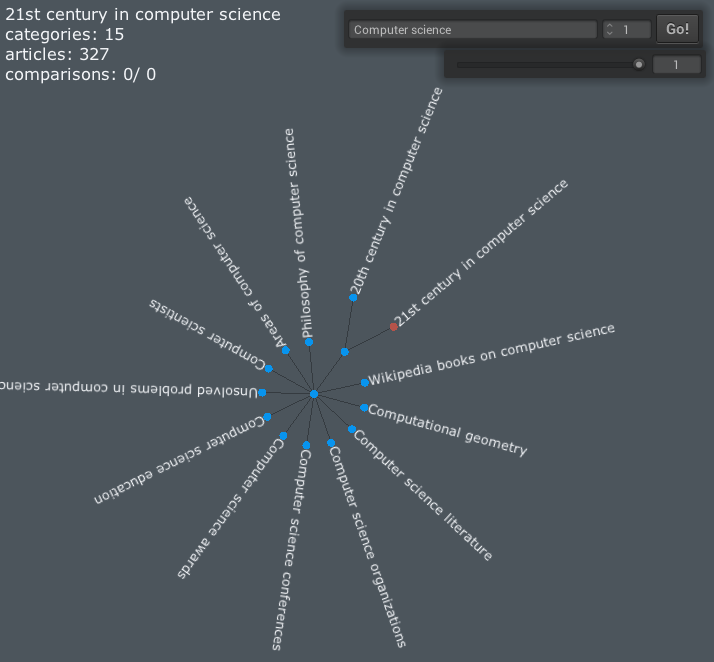
\includegraphics[scale=.21]{images/rotation-hist-2}&[3mm]&
        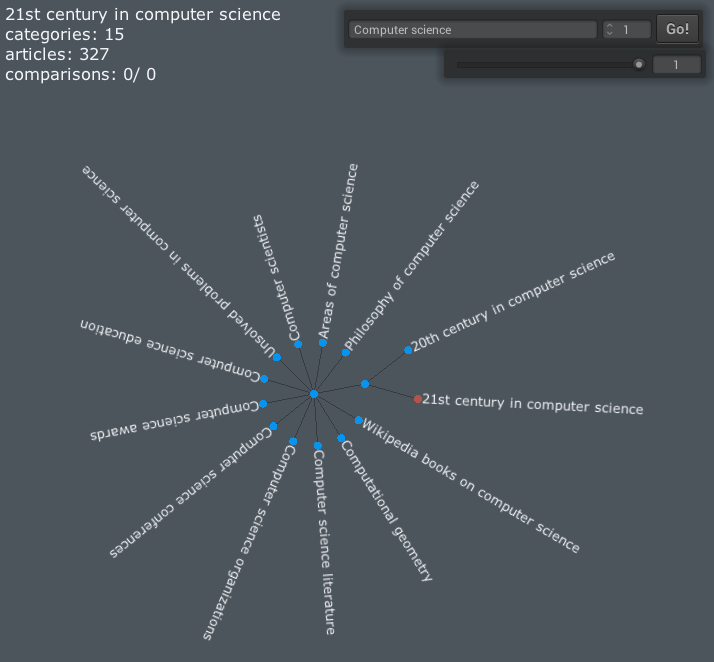
\includegraphics[scale=.21]{images/rotation-hist-3}\\
    };
    \draw[-{Latex[length=3mm]}] (m-1-1) -- (m-1-3);
    \draw[-{Latex[length=3mm]}] (m-1-3) -- (m-1-5);
    \end{tikzpicture}
    \caption{Der Kategoriebaum für die Wurzelkategorie \emph{Computer science} und der expandierten Unterkategorie \emph{History of computer science} wird um 90\textdegree Grad im Uhrzeigersinn gedreht.}
    \label{fig:rotation-tree}
\end{figure}

% zwei Bilder mit Pfeil Drehung der Kategorie
Platziert der Nutzer den Mauszeiger über einer bestimmten Kategorie, wird ihm deren Titel in der zusammenfassenden Statistik angezeigt, wie in Abbildung \ref{fig:small-start} gezeigt.
Somit ist es auch möglich, sich Titel von Kategorien, die keine Blattkategorien sind, anzeigen zu lassen, ohne dass sich die gezeichneten Elemente überlagern.

Die essenzielle Interaktion mit der Visualisierung ist die Expansion ausgewählter Kategorien.
Die Expansion einer Kategorie wird durch einen Doppelklick auf die Kategorie ausgeführt.
Dabei werden die Unterkategorien der Ausgangskategorie dem Kategorienbaum hinzugefügt und als Knoten in die Visualisierung gezeichnet.
Die neuen Unterkategorien werden durch Kanten mit der Ausgangskategorie verbunden.
Dies wird in Abbildung \ref{fig:expand-cat} verdeutlicht.
Die Expansion ermöglicht dabei dem Nutzer, einen bestimmten Pfad von Unterkategorien schrittweise zu erkunden.
Die Erkundung der Unterkategorien eines Themengebiets wird dadurch differenzierter. 
Neben der Expansion des Kategorienbaums für alle Blattkategorien, durch das Eingabefeld für die Tiefe, wird zudem eine feinere Interaktion zur Verfügung gestellt.
Die Erweiterung einer Kategorie ist als eine inhaltliche Vertiefung zu verstehen.
Das hinzufügen von Unterkategorien zu dem Kategorienbaum stellt eine Spezifizierung des umschriebenem Gegenstand der Ausgangskategorie dar.
Diese Spezifizierung des umschriebenen Gegenstands, durch die Unterkategorien, wird in dieser Arbeit als inhaltliche Vertiefung festgelegt.
Die Expansion stellt dabei immer eine Spezifizierung der Abstraktionsebene dar, da nur Unterkategorien dem Kategorienbaum hinzugefügt werden können.

\begin{figure}
    \centering
    \begin{tikzpicture}
    \matrix (m) [matrix of nodes, nodes in empty cells] %, row 1/.style={nodes={minimum height=90mm}}]
    {
        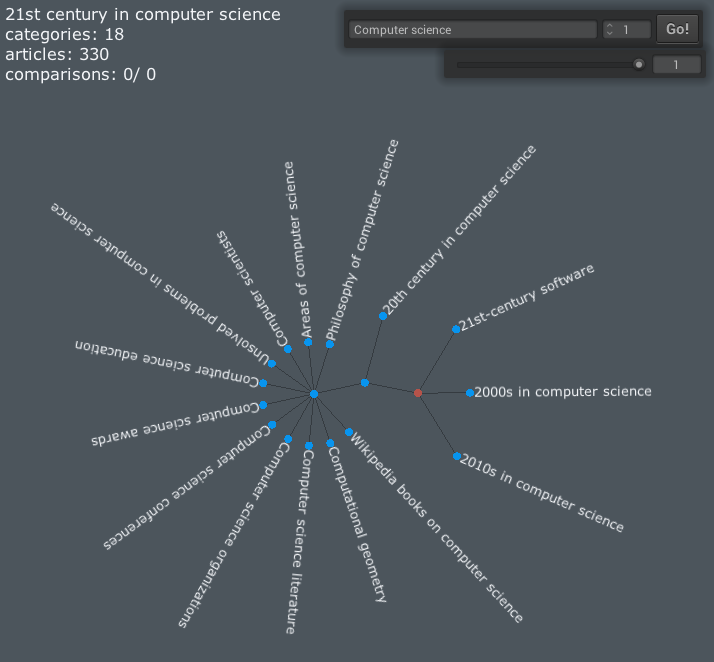
\includegraphics[scale=.3]{images/expand-hist/expand-hist-3.png}&[3mm]&
        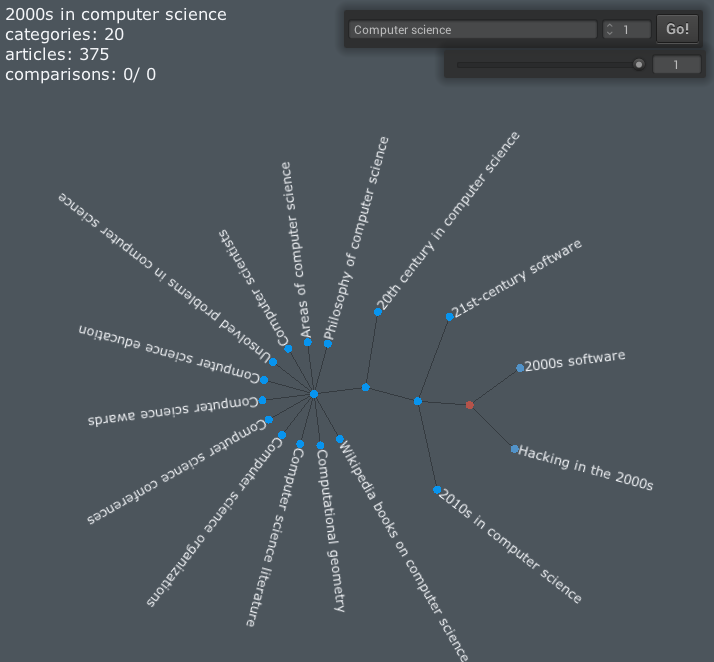
\includegraphics[scale=.3]{images/expand-hist/expand-hist-4.png}&[3mm]&\\
    
        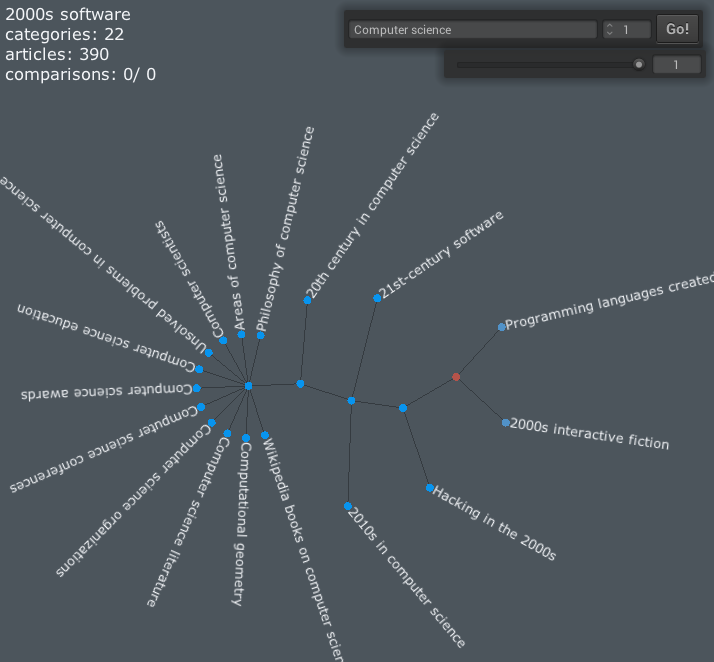
\includegraphics[scale=.3]{images/expand-hist/expand-hist-5.png}&[3mm]&
        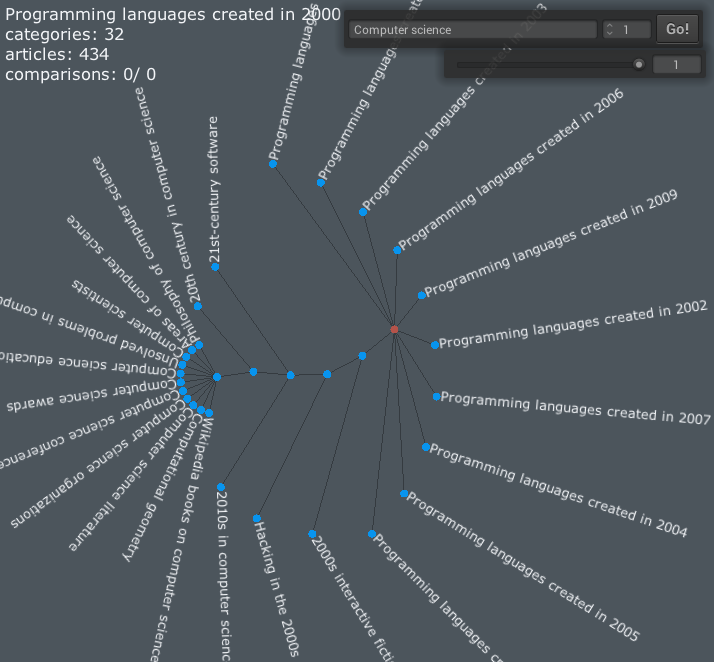
\includegraphics[scale=.3]{images/expand-hist/expand-hist-6.png}&[3mm]\\
    };
    \draw[-{Latex[length=3mm]}] (m-1-1) -- (m-1-3);
    % \draw[-{Latex[length=3mm]}] (m-1-3) -- (m-1-3);
    \draw[-{Latex[length=3mm]}] (m-2-1) -- (m-2-3);
    \end{tikzpicture}
    \caption{Die Bildabfolge stellt mehrere Expansionen von Unterkategorien der Kategorie \emph{History of Computer science} dar. Die expandierten Kategorien sind rot gefärbt.}
    \label{fig:expand-cat}
\end{figure}

Mit einem einfachen Klick auf eine Kategorie, wird die Kategorie rot gefärbt, damit diese von anderen Kategorien unterschieden werden kann.
Diese Auswahl einer Kategorie ergibt, in Kombination mit der Änderung des Schwellwerts, eine neue Interaktion.
Durch die Fokussierung der Kategorie werden Kategorien nur dann gelb gefärbt, wenn sie zwei Bedingungen erfüllen:
1. Unter den Kategorien müssen Artikel eingetragen sein, die eine Ähnlichkeit zur fokussierten Kategorie aufweisen. Diese Ähnlichkeit muss darüber hinaus über dem Schwellwert liegen.

\begin{figure}
    \centering
    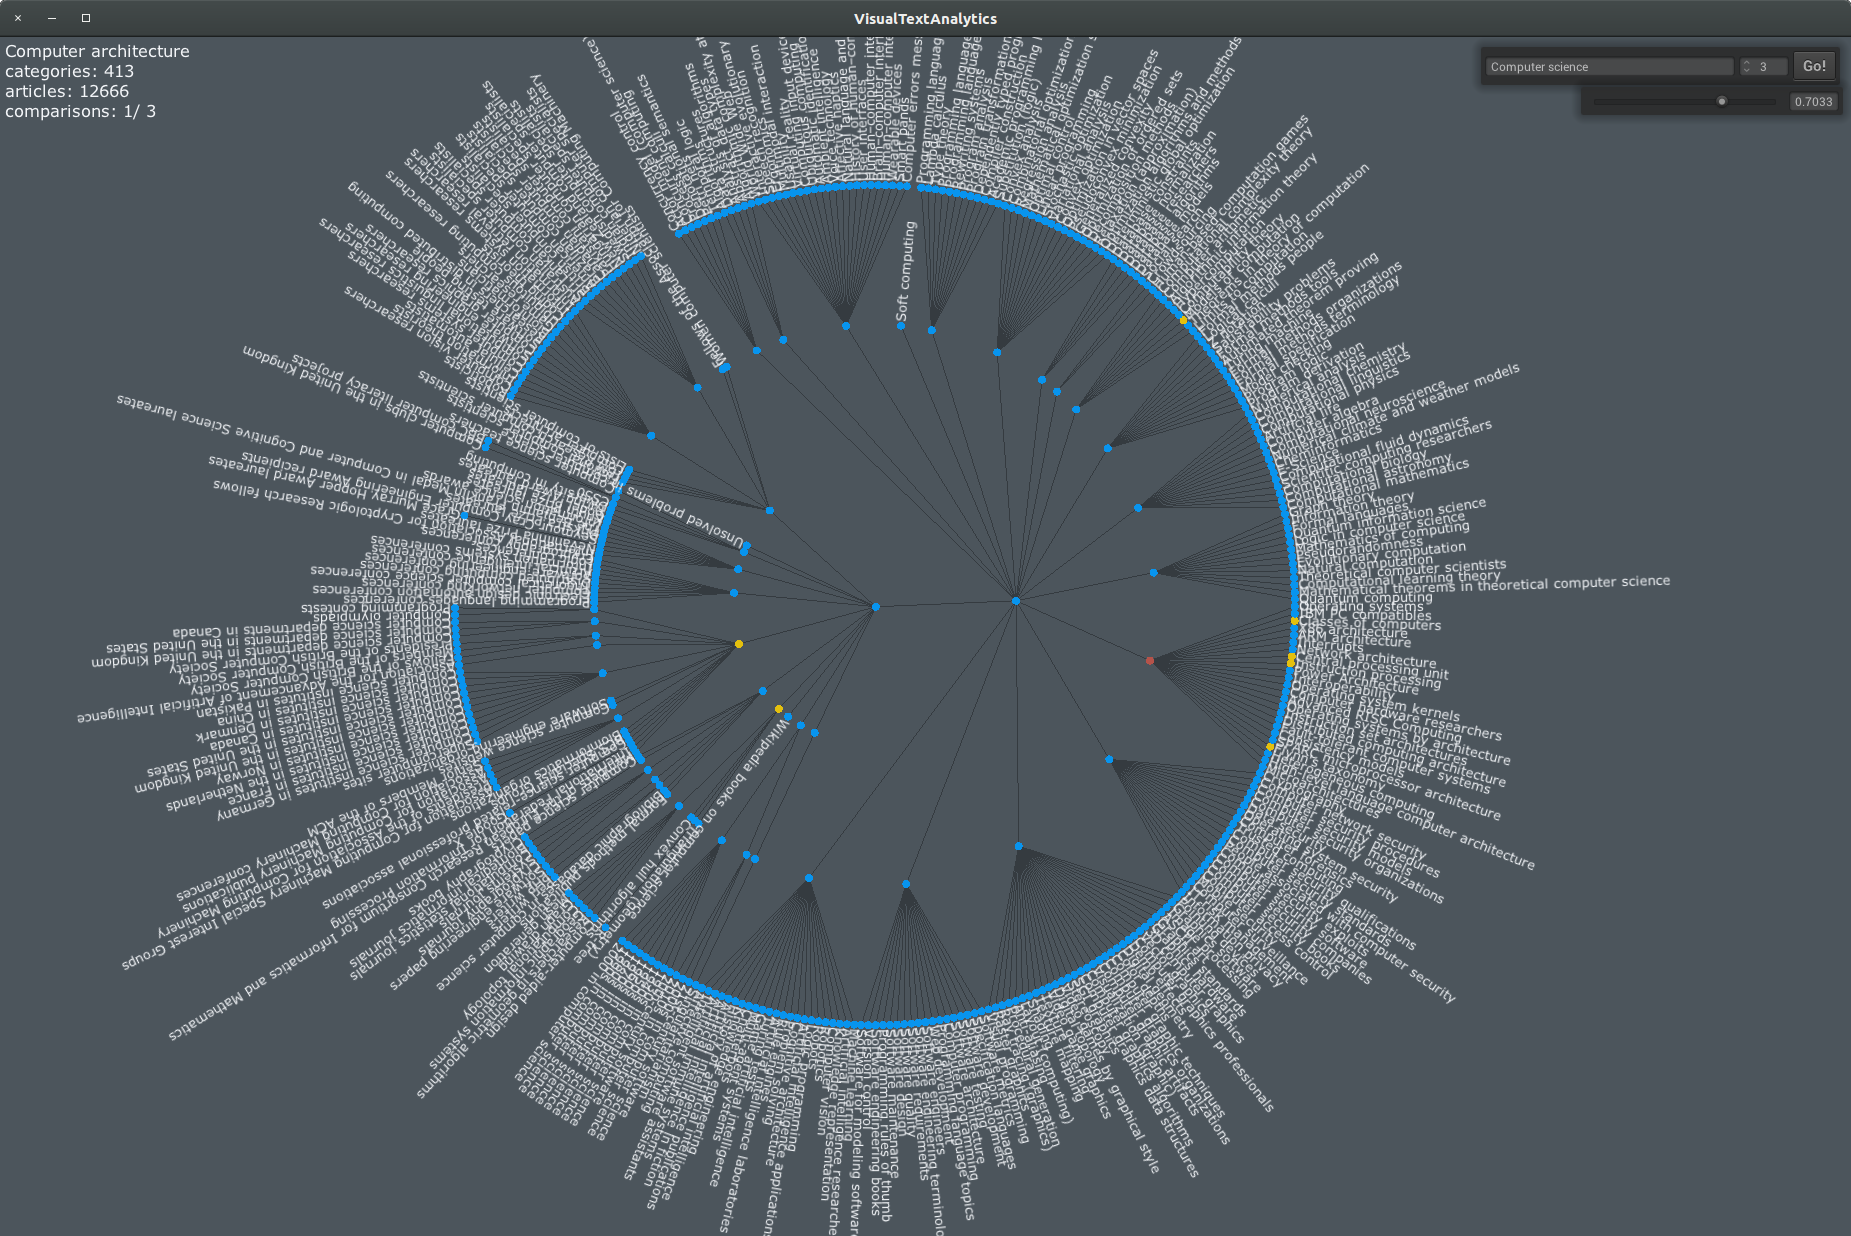
\includegraphics[width=\textwidth]{images/threshold-7033-lvl3-focus}
    \caption{Die rot gefärbte Kategorie \emph{Computer architecture} wurde fokussiert. In den gelb gefärbten Kategorien sind Artikel mit einer Ähnlichkeit zur rot gefärbten Kategorie eingetragen. Der Ähnlichkeitswert eines Artikelpaares zwischen zwei Kategorien liegt mindestens bei $0.7033$}
    \label{fig:threshold-focus-cat}
\end{figure}


\section{Filterung der "Ahnlichkeitsmatrix} \label{subchap: filter-vis}

% In diesem Abschnitt soll die Grafik über die simMatrix als abstraktes, nicht sichtbares Datenmodell dargestellt werden!!!
Dieses Kapitel beschäftigt sich mit, dass, durch die Interaktion mit der Darstellung, auch der Inhalt der Ähnlichkeitsmatrix aus Kaptiel \ref{subchap:simmatrix} verändert wird.
In der Einleitung dieses Kapitels wird erwähnt, dass der Kategorienbaum als Hierarchie von Abstaktionsebenen interpretiert wird und die Exploration von Kategorien nach einer \emph{Top-Down}-Herangehensweise realisiert wird.
Für die Dauer einer Darstellung des Kategorienbaums werden auch die Informationen über Ähnlichkeiten von Artikeln verfügbar gemacht.
Artikel, die in einer der dargestellten Kategorien eingetragen sind, werden mit Ähnlichkeiten zu anderen Artikeln in den Hauptspeicher geladen und als Matrix gespeichert.
Auf diese Weise entsteht eine neue, kleinere Ähnlichkeitsmatrix.
Die Ähnlichkeitsmatrix wird dabei auf Basis der ausgewählten Menge an Kategorien vertikal gefiltert.
Dies bedeutet, dass Zeilen aus der ursprünglichen Matrix verworfen werden.
Dies veranschaulicht Abbildung \ref{fig:simM-threshold-cat}.
Das verwendete Verfahren wird \emph{kategorienbasierte} Filterung oder \emph{vertikal} Filterung genannt.
Expandiert ein Nutzer eine Kategorie, um ihre Unterkategorien zu untersuchen, wird die Ähnlichkeitsmatrix um die Artikel aus den Unterkategorien vertikal erweitert.
Artikel und ihre Ähnlichkeitswerte sind somit, wie Kategorien, dynamisch verfügbar.

Die Menge an Artikel die durch bestimmte Kategorien, dargestellt in der Visualisierung als Kategorienbaum, ausgewählt werden, werden Kategorienraum genannt. 
Der Kategorienraum stellt auf Artikelebene die Thematische Ausbreitung des Kategorienbaums dar.
Durch die Einführung  des Kategorienraums ergibt sich eine neue interessante Sichtweise auf die Artikelähnlichkeiten.

 
In der Ähnlichkeitsmatrix, welche durch eine Auswahl an Kategorien durch den Kategorienbaum entsteht, werden Artikel mit allen Ähnlichkeiten zu anderen Artikel 
Die Artikel die innerhalb des Kategorienraums Ähnlichkeiten besitzen werden \emph{lokale} Vergleiche genannt.
Die Artikelpaare die einen Artikel enthalten, welcher nicht im Kategorienraum  
In der Abbildung soll verdeutlicht werden wie sich \emph{lokale} und \emph{globale} Vergleiche in der Ähnlichkeitsmatrix unterscheiden
Durch den neuen Ansatz können Ähnlichkeiten zwischen Artikel innerhalb oder außerhalb des Kategorienraums liegen.
Dies geben die zwei Werte der Zeile \emph{comparisons} aus dem Element (c) der Abbildung \ref{fig:small-start} wieder.

\begin{figure}
    \begin{tikzpicture}
    \end{tikzpicture}
    
\includegraphics{images/todobild}
    \caption{Darstellung einer Filterung der Ähnlichkeitsmatrix, die durch den Schwellwert entsteht}
    \label{fig:simM-threshold-cat}
\end{figure}

Eine weitere Methode, um die Größe der Ähnlichkeitsmatrix zu reduzieren, ist die \emph{horizontale} Filterung.
Diese Strategie der Reduzierung der Ähnlichkeitsmatrix ist über die Verschiebung des Reglers des Schwellwertes möglich.
Werden die betrachteten Ähnlichkeitswerte durch einen festgelegten Schwellwert begrenzt, verkürzen sich die Zeilen der Ähnlichkeitsmatrix.
Dieser wird in Abbildung \ref{fig:simM-threshold-cat} grafisch dargestellt.\\

Eine Kombination aus einer vertikalen und einer horizontalen Filterung entsteht, wenn eine Kategorie über einen festgelegten Schwellwert, wie im vorangegangenem Abschnitt beschrieben, fokussiert wird.
In Abbildung \ref{fig:simM-threshold-focus-cat} wird dargestellt, auf welche Weise sich diese Interaktion in der Ähnlichkeitsmatrix abbildet.
Durch die Fokussierung einer Kategorie die Artikel mit Ähnlichkeiten über einem festgelegtem Schwellwert enthält, wird die Ähnlichkeitsmatrix weiter gefiltert.
Auf diese Weise werden nur Artikelpaare betrachtet von denen die mindestens einer der beiden Artikel in der fokussierten Kategorie eingetragen sein muss.
Die Ähnlichkeitsmatrix besteht an dieser Stelle nur noch aus Artikeln, die in der fokussierten Kategorie eingetragen sind und ihren \emph{lokalen} Vergleichen zu anderen Artikel aus dem Kategorienraum.
Zusätzlich erfolgt einer Filterung der Ähnlichkeiten die unter dem Schwellwert liegen.
Diese Herangehensweise soll eine weiter Möglichkeit zur Filterung bereitstellen und eine Analyse der Daten vereinfachen.

\begin{figure}
    \begin{tikzpicture}
    \end{tikzpicture}
    
\includegraphics{images/todobild}
    \caption{Darstellung der Filterung der Ähnlichkeitsmatrix, die durch den Schwellwert entsteht, in Kombination mit einer fokussierten Kategorie}
    \label{fig:simM-threshold-focus-cat}
\end{figure}








% Wird eine Zahl eingegeben, die kleiner ist als die letzte angegebene Tiefe?
% Ein Nutzer gibt in der Suchleiste den Namen einer Kategorie ein, dabei wird im Hintergrund die Datenbank mit allen Wikipedia-Kategorien nach der Existenz der gesuchten Kategorie überprüft.
% Entspricht der gesuchte Begriff nicht einer Wikipedia-Kategorie wird der Nutzer aufgefordert, einen neuen Suchbegriff einzugeben.
% Die Schaltfläche "`GO"', rechts von der Suchleiste angeordnet, wird rot gefärbt, um darauf aufmerksam zu machen, dass die Suche erfolglos war. 
% Abbildung~\ref{fig:wrong-cat} zeigt die Suchleiste mit rot gefärbter Schaltfläche.

% =============================

% Notizen ingnorieren =================
% Ebene --> ringe!!
% Warum ein radiales Layout? warum konzentrisch, Welche Eigenschafte  sind gefragt und welche werden erfüllt.
% Ausnutzen des gesamte Raums?
% Konkrete Struktur des Kategorienbaums ist nicht klar.

% Wie funktioniert der Algorithmus von Eades?
% fokus aug Knoten statt Kanten.
% Strategie der beschriftung der Knoten.
%  ====================================



%Der Schieberegler ändert an erster Stelle nicht den sichtbaren Schwellwert, sondern gibt eine Grenze für die Artikelähnlichkeit den Datensatz an.




% An verschiedenen Stellen in diesem Kapitel wurde darauf verwiesen, dass die Darstellung des Kategorienbaums Auswirkungen auf den Inhalt der  Ähnlichkeitsmatrix, welche in  Kapitel \ref{subchap:simmatrix} beschrieben wurde, hat.
% Dieser Abschnitt beleuchtet die Vorgänge mit der die Ähnlichkeitsmatix gefiltern werden kann.
% Ziel neben der Darstellung  des Kategorienbaums, ist die Filterung der Ähnlichkeitesmatrix.
% Wie in der Einleitung 




% \begin{itemize}
%     \item Erl"auterung der Auswahl von Artikel aus der "Ahnlichkeitsmatrix
% \end{itemize}



% %% Kapitel Visualisierung realisiesrung
% Der Datensatz über die Ähnlichkeiten zwischen den Artikeln soll im Hintergrund auf diejenigen Artikel reduziert werden, welche den explorierten Kategorien entsprechen.
% Auf diese Art soll die Matrix mit mehreren Billionen Vergleichen nicht nur auf eine überschaubare Menge reduziert werden, die klein genug ist, um sie schnell zu verarbeiten, sondern auch auf ein Themengebiet eingeschränkt werden.
% Der Grundgedanke ist dabei, dass die Nachvollziehbarkeit von Ähnlichkeitswerten erleichtert wird, da sich die Artikel bereits thematisch ähneln und zudem eventuell ein ähnliches Vokabular benutzen.
% Die Vermutung liegt nahe, dass in einem abgeschlossenen Themengebiet die Vergleichswerte zwischen den Artikeln sehr hoch sein werden.




\chapter{Implementierung}
\label{chap:Implementierung}
% !TEX root = ../main.tex
% Implementierung



\section{Programm Struktur}
\begin{itemize}
    \item Klassen"ubersicht des Programms
    \item Programmablauf
    \item Erl"auterung der KernfFunktionen der einzelnen Klassen im Detail
\end{itemize}



\section{Externe Bibliotheken}
\begin{itemize}
    \item WikiDB
    \item NanoGUI
    \item NanoVG
\end{itemize}













\chapter{Zusammenfassung}
\label{chap:Zusammenfassung}
% Zusammenfassung



\section{Ausblick}















































































% draft concept

% \section{Konzept}
% Das Ziel der Visualisierung ist es, die Kosinusvergleiche zwischen Wikipedia-artikel darzustellen und F"alle von Textwiederverwendung aufzuzeigen.
% Die Daten zu den Artikeln sollen wenn möglich ohne lange Wartezeiten dargestellt werden k"onnen sowie weiter Informationen zu den Artikeln.


% \subsection{Visualisierung der Kategorien}
% Die Visualisierurng startet mit einer "Ubersicht der 22 "`Main Topic Classifications"'  und einer Suchleiste.

% Die 22 "`Main Topic Classifications"' sollen mit dem jeweiligen Namen der Kategorie als Knoten radial angeordnet werden. Im Zentrum des radialen Layouts soll die Suchleiste platziert werden.

% Die Gr"o"se der Knoten zeigt an, wie viele direkte Subkategorien in der Kategorie enthalten sind. 
% Eine weitere Möglichkeit w"are 
% es, die Gr"o"se der Kategorie Knoten auf die Anzahl aller direkten und indirekten Subkategorien abzubilden.
% In der Suchleiste kann nach einer beliebigen Kategorie gesuchen werden, damit wird die gewählte Kategorie in den Fokus der Visualisierung gestellt.
% Existiert zu dem Suchbegriff eine Kategorie wird der Titel der Kategorie im Zentrum der Visualisierung dargestellt.
% Auf dem radilem Layout werden die 22 "`Main Topic Classifications"' ersetzt, durch die direkten Subkategorien der gefundenen Kategorie.

% Wählt man mit einem Klick einer der Kategorien aus, die im radialem Layout angeordnet sind, werden die direkten Subkategorien dargestellt.
% Auf diese Weise wird dem Nutzer erm"oglicht, den gerichteten Kategoriegraphen, zu explorieren.
% Durch die nun zusätslich dargestellten Subkategorien lässt sich ein Überblick gewinnen, in welchen Kategorien besonders viele Artikel stehen.
% % Um noch nicht sichtbare Verkn"upfungen zwischen Kategorien aufzuzeigen, w"are es m"oglich die Kanten des gerichteten Graphen einzublenden, welche in der Logik der Kategorien Hierarchie auf Kategorien zeigen, welche h"ohre liegen.

% \paragraph{Filter}

% An diesem Punkt wäre eine M"oglichkeit der weiteren Interaktion die Benutzung verschiedener Filter auf den sichtbaren Kategorien.
% Die Filterfunktionen sollen es ermöglichen, anhand von ausgewählten Eigenschaften, nur noch bestimmte Kategorien darzustellen.
% Möchte der Nutzer nur die Kategorien mit besonders langen Artikeln sehen, kann er nach der Artikellange filtern. Weitere m"ögliche Filter wären zum Beispiel:
% \begin{itemize}
%     \item Anzahl der enthaltenen Artikel 
%     \item Anzahl der Paragraphen
%     \item Anzahl der entahltenen Sub-Kategorien
% \end{itemize}

% Denkbar sind jedoch alle zur Verf"ugung stehenden Informationen über Artikel und Kategorien.
% In den Kategorien stehen Artikel, welche einer genauen Revision zugeordnet werden können. Die Revision stellt ein Änderung am Artikel dar
% und lässt sich einem Revisioner, einer Uhrzeit an dem die Änderung stattgefunen hat und evtl. sogar einem Standort zuordnen.
% Nach solchen Eigenschaften lie"sen sich die Kategorien auch filtern.

% \paragraph{"Ahnlichkeitsmatrix}

% Um die dargestellten Kategorien in Bezug zueinander zu stellen, werden weitere Informationen ben"otigt, welche nicht direkt aus der 
% Wikipedia kommen k"onnen. Dazu ist der Datensatz mit Kosinus-Vergleichen n"otig.

% Durch die Auswahl einer Kategorie, wird auch gleichzeitig die Menge, der in ihr enthaltenen Artikel ausgew"ahlt.
% Wenn man sich alle Kanten zwischen den Artikeln anzeigen lassen würde, welche eine "Anlichkeit zu einander haben, hätte man ein klassisches "Overplotting" Problem und w"urde nichts mehr erkennen.

% Wählt man eine Kategorie aus, die einen Interessiert sucht ein Algorithmus aus der Menge an Artikeln der gew"ahlten Kategorie und den restlichen Artikel in den anderen Kategorien,  Pärchen, die einen "Ahnlichkeitswert aufweist, der "uber einem festgelegten Schwellwert liegt.
% Die nicht ausgew"ahlten Kategorien werden je nach Anzahl der enthaltenen Treffer unterschiedlich stark gef"arbt.
% In der Visualisierung erkennt man nun, in welchen Kategorien Artikel "Ahnlichkeiten zueinander haben und ob viele dieser Verbindungen zwischen den Kategorien existieren.
% Sind zwei Kategorien ausgew"ahlt wird eine andere Form der Visualisierung gebraucht, um die zwei Kategorien darzustellen.


% \subsection{Visualisierung der Artikel}
% In einem vorherigem Schritt wurden zwei Kategorien ausgew"ahlt, welche Artikeln mit "Ahnlichkeiten "uber einem bestimmten 
% Schwellwert zueinander besitzen.
% In dieser Visualisierung m"ochte man auf die Artikel und deren Relation zueinander eingehen. 

% Der Focus in diesem Teil der Visualisierung sollte auf den Artikeltexten und Passagen von Textwiederverwendung liegen.
% Zu sehen sind zwei Listen von Paragraphen, getrennt durch eine Art Lineal, welches den "Ahnlichkeitswert angibt.
% Alle Paragraphen tragen als "Uberschrift den Titel aus dem Artikel aus dem sie stammen.
% In der linken Liste sind die Paragraphen, aus der Referenzkategorie und in der rechten h"alfte sind die Paragraphen aus der 
% vergleichenden Kategorie.
% Es sind alle Paragraphenp"archen aus den zwei Kategorien geladen, durch scrollen ist es m"oglich weiter P"archen mit einer niedrigeren 
% "Ahnlichkeit zu sehen.

% Mit einem Klick auf einen gelisteten Paragraphen, werden die restlichen Paragraphen aus dem zugehörigem Artikel in der Listenansicht dargestellt.
% In der Listenansicht der referenzierten Kategorie ist nun ein kompletter Artikel, mit all seinen Paragraphen dargestellt.
% Nun kann sich angeschaut werden zu welchen weiteren Paragraphen, au"serhalb der gewählten Kategorie, der Artikel Ähnlichkeiten besitzt.
% Die neue Auflistung an Paragraphenpärchen ist wieder nach absteigender Ähnlichkeit sortiert, jedoch ist es auch möglich den Artikel seiner
% ursprünglichen Reihenfolge darszustellen.

% Zwischen zwei "ahnlichen Paragraphen kann ein Textalignment berechnet werden um die Artikel weiter zu inspizieren und herauszufinden,
% ob Textpassagen in beiden Paragraphen verwendet wurden.


% Zu Beginn sieht man die 22 Main Tonic Classifications
% Jede Main Topic Classification wird als Knoten dargestellt
% die Größe des Knoten ist abhängig von der direkten Anzahl an Artikel in der Kategorie
% die 22 Main Topic Classifications sind radial angeordnet
% in dem radialem Layout ist eine Suchleiste, mit der sich nach weitern Kategorien suchen lässt
% alle Kategorien die auf dem radialem Layout angeordnet sind lassen sich durch eine klick expandieren
% expandierte Kategorien zeigen ihre direkten Subkategorien an
% es lassen sich mehrere Kategorien und Subkategorien zeitgleich expandieren
% auf allen sichtbaren Kategorien lassen sich Filter anwenden
% Filtern lassen sich die Kategorien nach mehreren Eigenschaften
% \begin{itemize}
%     \item Anzahl der enthaltenen Artikel 
%     \item Anzahl der Paragraphen
%     \item Anzahl der entahltenen Sub-Kategorien
%     \item Anzahl der Wörter
% \end{itemize}


% Eine Kategorie kann ausgewählt werden, dadurch werden alle anderen Kategorien auf Ihre Ähnlichkeit hin eingefärbt
% verglichene Kategorien werden nach Anzahl der Ähnlichkeitspärchen unterschiedlich start eingefärbt
% ein Schwellwert kann eingestellt werden, ab welchem Ähnlichkeitswert Artikelpaare in Betracht gezogen werden.



% \section{Daten}

% % ////////////////////////////////////
% \begin{figure}[H]
%     \centering
%     \begin{subfigure}[b]{0.96\textwidth}
%         \includegraphics[width=\textwidth]{images/01_introduction/motivation_temporal_superresolution_one.pdf}
%         \caption{3D video playback rate matching the low recording rate}
%         % \label{subfig:playback_rate_matching}
%     \end{subfigure}
    
% 	\vspace{1.0cm}
    
%     \begin{subfigure}[b]{0.96\textwidth}
%         \includegraphics[width=\textwidth]{images/01_introduction/motivation_temporal_superresolution_two.pdf}
%         \caption{3D video playback matching the video encoding standards to ensure persistence of fluid motion}
%         % \label{subfig:playback_rate_higher}
%     \end{subfigure}
%     \caption[Concept of Temporal Super Resolution in a 3D Video Player]{In this Figure, two different playback rates for a low frame rate recording of a 3D volume sequence is presented. The tick marks on the black arrows indicate the position of recorded frames. The blue arrows indicate the playback rate that matches the recording \subref{subfig:playback_rate_matching} and an increased playback rate \subref{subfig:playback_rate_higher} using temporal interpolation to provide the viewer with a impression of fluid motion. }
%     % \label{fig:temporal_superresolution}
% \end{figure}

\cleardoublepage
\clearpage
%
%\chapter{Future Work}
%\label{chap:future_work}
%\input{sections/09_future_work.tex}


% ================================================================


% \newpage
% \let\cleardoublepage\clearpage
% \chapter*{Danksagung}
% The \textit{Lena} image is obtained from the website of Mike Wakin\footnote{ \textit{Lena} test image website.\quad {\url{http://www.ece.rice.edu/~wakin/images/}}\newline [Online, accessed 26-November-2016]}.

% Wikipedia Datensatz

% Ähnlichkeitsmatrix Tristan Licht

% wikidb project visaul text analytics


% ================================================================


%\pagebreak
%\hspace{0pt}
%\vfill

% \chapter*{}
% \todo{perso"hnliche Danksagung}

% ================================================================

%\vfill
%\hspace{0pt}
%\pagebreak

%\printglossary[type=\acronymtype]

%alphadin_martin
%\bibliographystyle{bibliographie/a_m.bst}
\bibliographystyle{unsrt}
{\footnotesize
\bibliography{bibliographie/bibliographie}
}

% ================================================================


\newpage
% Anhang
% %\begin{multicols}{2}
% \begin{appendices}
% \addchap{Appendices}
% \chapter{Pseudocode}
% \label{app:pseudocode}
% \begin{algorithm}[H]
\SetAlgoLined
    \SetKwProg{Fn}{Function}{}{}
    \SetKwInOut{Input}{input}
    \SetKwInOut{Output}{output}

    
\Fn{compute\_cw\_offset(c$_i$, dims$_{codeword}$, $dims_{codebook}$)}{

\Input{an integer $c_i$ indexing a codeword, the 3D codeword and codebook texture dimensions $dims_{codeword}$ and $dims_{codebook}$}
\Output{a 3D integer vector $offset_{codeword}$ indicating the codeword offset in the texture}

\BlankLine

\BlankLine

$num\_codewords_{xy}$ $\gets$ $dims_{codebook_{xy} }$ $\mathbf{div}$ $dims_{codeword_{xy} }$   \Comment{component-wise division}

$num\_codewords_{slice}$ $\gets$ $num\_codewords_x$ * $num\_codewords_y$ \Comment{number per texture slice}

\BlankLine

$offset_{codeword{_z}}$ $\gets$ $c_i$ $\mathbf{div}$  $num\_codewords_{slice}$ \Comment{compute z offset of codeword}
 
 
$c_i$ $\gets$ $c_i$ - $num\_codewords_{slice}$ \Comment{reduce index by z offset}
  
$offset_{codeword{_y}}$ $\gets$ $c_i$ $\mathbf{div}$  $num\_codewords_{x}$ \Comment{compute y offset of
 codeword}
 
$offset_{codeword{_x}}$ $\gets$ $c_i$ $\mathbf{mod}$ num\_codewords$_{x}$ \Comment{compute x offset of codeword}  

\BlankLine

\Return $offset_{codeword}$
 
}
 \caption{Compute Integer Codeword Offset}
 \label{algo:codeword_offset}
\end{algorithm}


\newpage


\begin{algorithm}[H]
\SetAlgoLined
    \SetKwProg{Fn}{Function}{}{}
    \SetKwInOut{Input}{input}
    \SetKwInOut{Output}{output}

    
    %dims$_{idx}$, dims$_{codeword}$, $dims_{codebook}$)

\Fn{transform\_to\_ncs($p$,  $dims_{idx\_vol}$)} {
\Input{ a sampling position $p$ in normalized volume space, the index volume dimension
s $dims_{idx\_vol}$}

\Output{a sampling position relative to the dimensions of a codeword}

\BlankLine

\BlankLine

$p_{abs_idx}$ $\gets$ $p$ * $dims_{idx\_vol}$ \Comment{express position absolute number of codewords covered}

$p_{ncs}$ $\gets$ $get\_fractional(p_{abs_idx})$ \Comment retrieve fractional part

\Return $p_{ncs}$

}


\Fn{sample\_vq\_element($p$, $\hat{V}_{idx}$, $\hat{V}_{cb}$, $dims_{codeword}$) }{

\Input{ a sampling position $p$ in normalized volume space, the index volume $\hat{V}_{idx}$ and corresponding 3D codebook $\hat{V}_{cb}$, the dimensions of a 3D codeword $dims_{codeword}$ }

\Output{a decompressed sample $\hat{V}(p)$ being the reconstruction of $V(p)$}

\BlankLine

\BlankLine

$dims_{idx\_vol}$ $\gets$ $get\_dimensions(\hat{V}_{idx}$) \Comment{retrieve index volume dimensions}

$dims_{codebook}$ $\gets$ $get\_dimensions(\hat{V}_{cb}$) \Comment{retrieve codebook dimensions}

\BlankLine

$c_i$ $\gets$ $sample\_texture\_normalized(\hat{V}_{idx}$, $p$) \Comment{sample codeword idx in $\hat{V}_{idx}$ at $p$}

$offset_{codeword}$ $\gets$ $compute\_cw\_offset$($c_i$, $dims_{codeword}$, $dims_{codebook}$) \Comment{get int offset}

$offset_{element_l}$ $\gets$ $transform\_to\_ncs$($p,  dims_{idx\_vol}$) \Comment{get local offset to cw element}

$offset_{element_g}$ $\gets$ $offset_{codeword}$ + $offset_{element_l}$ \Comment{compute global offset}

\BlankLine

$vq\_decompressed\_sample$ $\gets$ $sample\_texture\_unnormalized$($\hat{V}_{cb}$, $offset_{element_g}$)

\BlankLine

\Return $vq\_decompressed\_sample$

 
% \While{While condition}{
 % instructions\;
 % \eIf{condition}{
  % instructions1\;
   %instructions2\;
   %}{
   %instructions3\;
  %}
 %}
}
 \caption{Sample Vector Quantized Element}
 \label{algo:vector_quantization_sampling}
\end{algorithm}







%  vec3 base_offset_plus_overflow = base_offset_fetch + overflow;



%  if( base_offset_plus_overflow.x >= current_index_texture_size.x ) {
%    overflow.x = 0;
%    padded_remaining_pos.x = clamped_reset_pos;
%  }

%  if( base_offset_plus_overflow.y >= current_index_texture_size.y) {
%    overflow.y = 0;
%    padded_remaining_pos.y = clamped_reset_pos;
%  }

%  if( base_offset_plus_overflow.z >= current_index_texture_size.z) {
%    overflow.z = 0;
%    padded_remaining_pos.z = clamped_reset_pos;
%  }


%  vec3 final_index_pos = base_offset_fetch + overflow;
%  final_index_pos = round(clamp(final_index_pos, vec3(0.0, 0.0, 0.0), vec3( current_index_texture_size ) - 1.0 ) )  ;
%  ivec3 int_index_pos = ivec3(final_index_pos);







% \end{appendices}
%
%\subsubsection*{cpu.c aus LinuxSiggraph 2011: Occlusion culling in Alan Wake 2.6.16}\label{•}.cpu}\lstinputlisting[language=C]%{code/cpu.c}
%\end{multicols}




\end{document}